\section{"Ubersicht verschiedener Barcodesysteme}
Zur Zeit befinden sich viele verschiedene Barcodesysteme in Benutzung. Manche sind spezifisch für einen bestimmten Wirtschaftszweig, andere wiederum findet man so gut wie überall. Dieser Abschnitt soll die bekanntesten und verbreitetsten Systeme vorstellen. Dabei wird eine Grobeinteilung anhand der Anzahl der Dimensionen des Codes vorgenommen.

\subsection{Eindimensionale Barcodes}
Eindimensionale Barcodes codieren Daten entlang ihrer Länge (also links und rechts); nicht ihrer Höhe (also oben und unten). Würde man nun eine Linie durch einen eindimensionalen Barcode ziehen, findet man diese Dimension. Dieses Vorgehen nutzen die meisten der verwendeten Laserscanner. Dass eindimensionale Barcodes meist sehr groß abgedruckt sind hat einen einfachen Grund: Je größer der Code, desto einfacher findet ihn ein Scanner.

\subsubsection{Strichcode}
\begin{figure}[htbp]
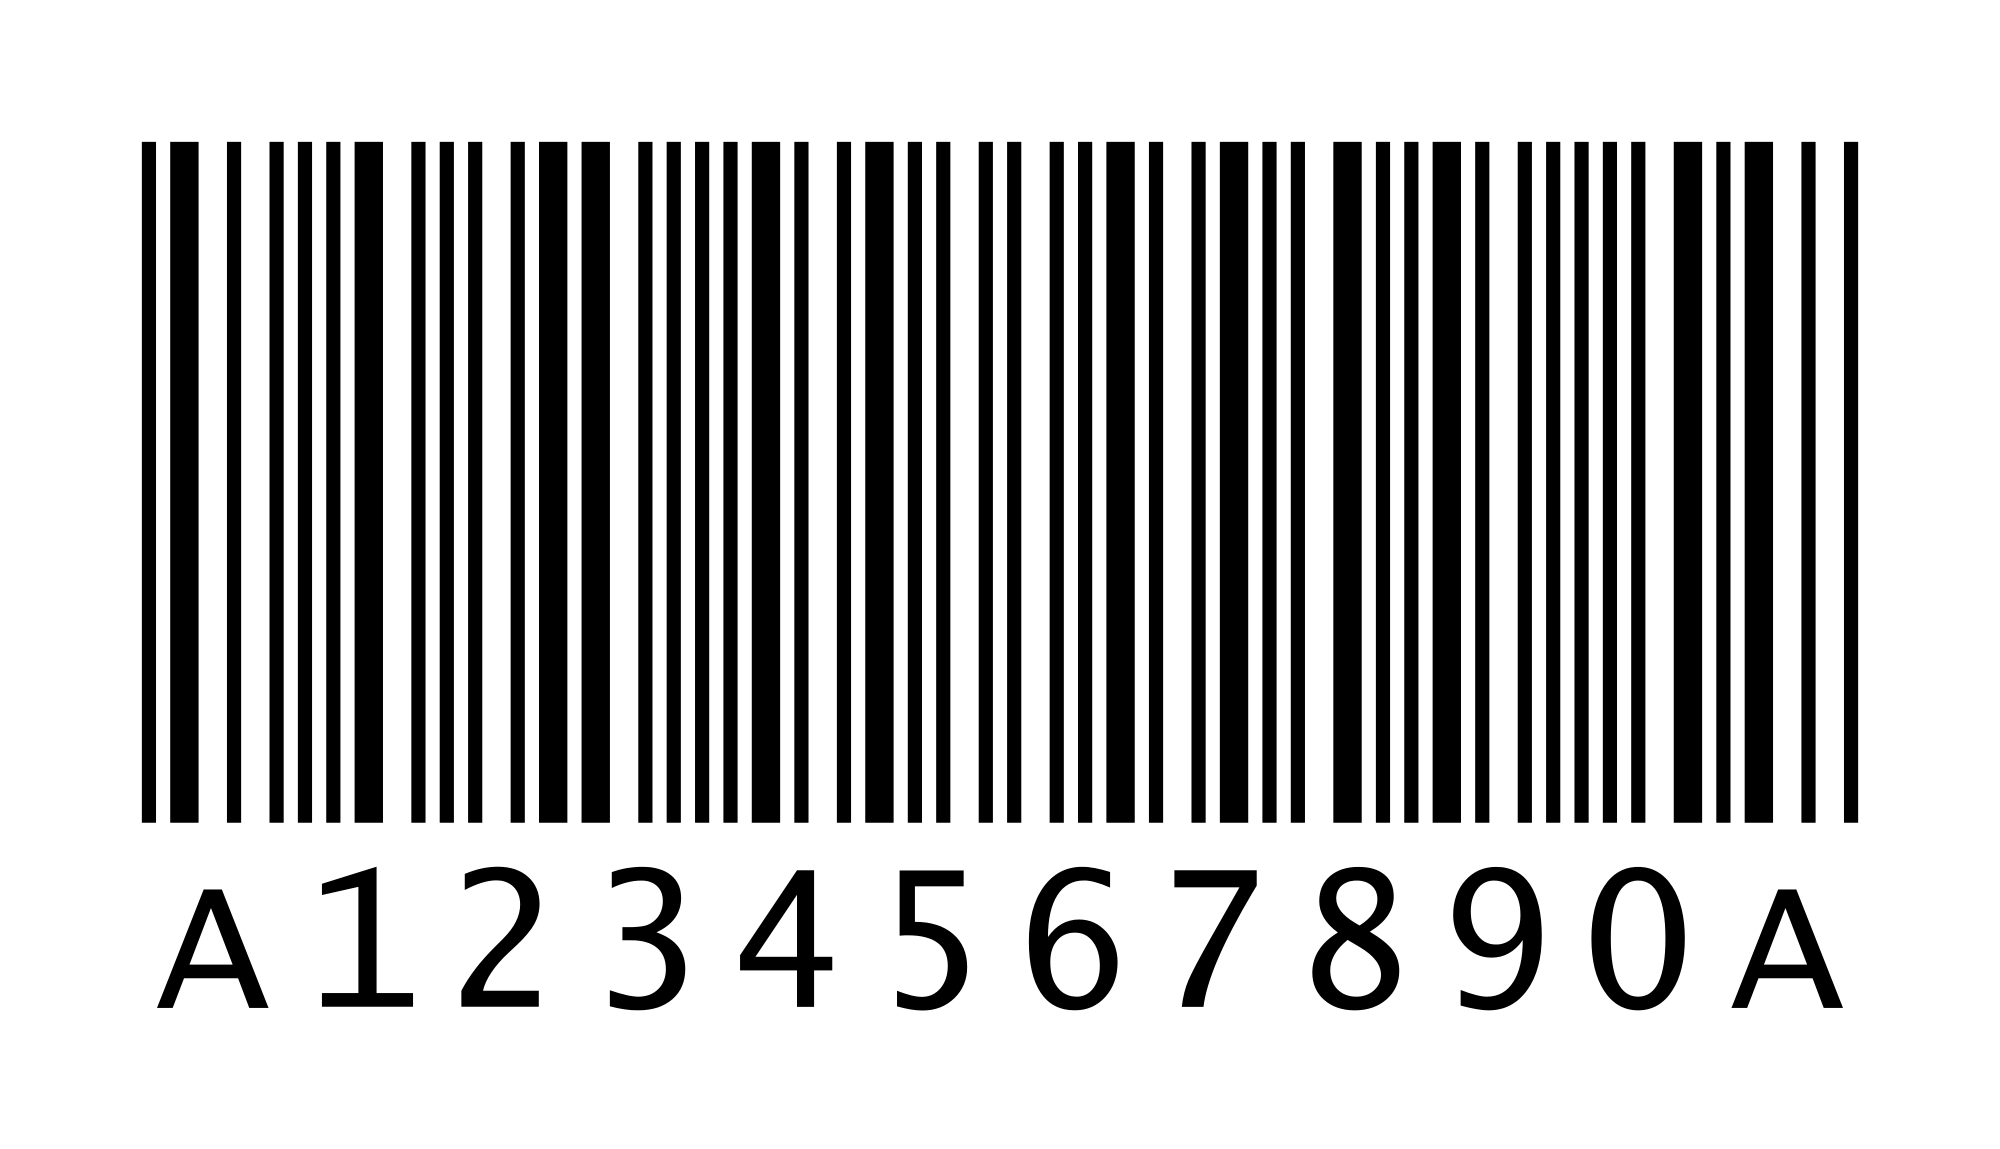
\includegraphics[height=2cm]{Bilder/Barcode.png}
	%\vspace{1cm}
	\caption{Barcode}
	\label{muffel}
\end{figure}

\subsection{sublorem}
Lorem ipsum dolor sit amet, consetetur sadipscing elitr, sed diam nonumy eirmod tempor invidunt ut labore et dolore magna aliquyam erat, sed diam voluptua. At vero eos et accusam et justo duo dolores et ea rebum. Stet clita kasd gubergren, no sea takimata sanctus est Lorem ipsum dolor sit amet. Lorem ipsum dolor sit amet, consetetur sadipscing elitr, sed diam nonumy eirmod tempor invidunt ut labore et dolore magna aliquyam erat, sed diam voluptua. At vero eos et accusam et justo duo dolores et ea rebum. Stet clita kasd gubergren, no sea takimata sanctus est Lorem ipsum dolor sit amet.
\pagebreak
